\documentclass[conference]{IEEEtran}
\IEEEoverridecommandlockouts
% The preceding line is only needed to identify funding in the first footnote. If that is unneeded, please comment it out.
\usepackage{cite}
\usepackage{amsmath,amssymb,amsfonts}
\usepackage{algorithmic}
\usepackage{graphicx}
\usepackage{textcomp}
\usepackage{float}
\usepackage{caption}
\graphicspath{ {./Images/} }
\usepackage[font=small,labelfont=bf]{caption}
\def\BibTeX{{\rm B\kern-.05em{\sc i\kern-.025em b}\kern-.08em
    T\kern-.1667em\lower.7ex\hbox{E}\kern-.125emX}}
\begin{document}

\title{Deep neural network for Bitcoin price prediction with tweet sentiment analysis\\
}

\author{\IEEEauthorblockN{Olivier Jérémy}
\IEEEauthorblockA{\textit{Master in Management, Business Analytics} \\
\textit{HEC Lausanne}\\
Lausanne, Switzerland \\
jeremy.olivier@unil.ch}

\and
\IEEEauthorblockN{Trillo Lago Luc}
\IEEEauthorblockA{\textit{Master in Finance, Data Science} \\
\textit{HEC Lausanne}\\
Lausanne, Switzerland \\
luc.trillolago@unil.ch}

\and
\IEEEauthorblockN{Granoux Aliaume}
\IEEEauthorblockA{\textit{Master in Finance, Data Science} \\
\textit{HEC Lausanne}\\
Lausanne, Switzerland \\
alliaume.granoux@unil.ch}
}

\maketitle

\begin{abstract}
Bitcoin is today one of the most popular assets for young people in the world, promises of untold riches for the new generation are tall and wide and rapidly everyone became an “expert” of cryptocurrencies and blockchain. This of course, got the “smart money” involved and these big players will try every strategy in the book and out of the box, to try to predict in which direction the price of Bitcoin will move and at what magnitude. It seems today that one of the most popular means of price prediction is sentiment analysis. Hedge funds, investment banks and others, will scout social media platforms, to find anything related to their investments and to find what people think of them. Out of this new complement of forecasting, one social media platform stands out, Twitter.
\end{abstract}

\begin{IEEEkeywords}
Bitcoin, Prediction, Sentiment analysis, Deep neural network
\end{IEEEkeywords}


\section{Introduction}
Social media has taken  the world by surprise over the last 10 years, it started slowly by being a means of communication between people over the world, and has since taken a more important part in our lives each day. We are now in a time where social media has taken a sharp change of direction, and where it has become a marketplace for corporations to find new customers and information on how to sell better. It has also become a way for people to influence each other's opinions, choices and lifestyles, meaning that people that may or may not be experts in a certain domain, can sway people’s opinions if their message is powerful enough or if they have a high enough notoriety that could reach a critical mass of people. This is used by many and for multiple purposes; trying to give importance to a topic that they find important like social problems; promoting products and reviewing them via influencers or ads in a more general way, democratizing knowledge that used to be hard to come by (this is something that was started by the internet in a more general way and exacerbated by social media),... all in all,social media is used in plentiful of ways, sometimes they are employed with a good intention in mind, sometimes not, but what is undeniable is that the effect that they have and have had in society is huge and this will keep with us for the foreseeable future.
\newline
\newline
Finance has always been a mysterious topic for the majority of people, some say that workers of the field make finance deliberately difficult to understand by inventing lingo so that people are deterred from interesting themselves in the field. Some find that the financial world is rather opaque and is mostly a form for rich people to keep being rich, others find the amount of money that circulates in this world obscene and many think that institutions of Wall Street are rampant with corruption and that they do not work in the interest of a nation or the people but rather are in the pocket of some individuals. This sentiment has been prevalent for decades, but has been even more democratized by the 2008 financial crisis and its mediatisation. 
\newline
\newline
Many of these reasons are why cryptocurrencies were created in the first place, people were trying to escape the roots of traditional finance and the regulations that governmental agencies chose-
During the aftermath of the crisis, new brokers appeared, these brokers proposed easily understandable financial tools, a variety of low cost index funds that attracted inexperienced people and people who did not want to go to extreme lengths to invest their money and even 0 commission trades, all these were crucial for what we know today as the democratization of investing. With this, a new community developed over the internet, a community focused on giving investing tips and picks. This community is very diverse today, with people ranging from inexperienced  to experts and giving great recommendations to extremely risky plays. 
\newline
\newline
These communities are today all over the place, Youtube, Reddit -and its infamous WallStreetBets-, Instagram, Twitter,... and even though they seem diverse, they are today what we call echo-chambers. Information gets repeated over and over without any type of scrutiny, opinions that differ from the perceived truth by the majority are labeled as disinformation or what they call “spreading FUD” -Fear, uncertainty and doubt– . This gives a disproportionate power to the biggest voices in the communities and these people do not always have the well being of the community at heart.
Another important characteristic of these communities, is that they are composed of mostly young people, of whom many grew within the “Meme” culture. This culture was brought with them into the investing world, giving us situations like Gamestop or AMC where an investment strategy was mostly based on a joke. Even though at first glance it may seem inoffensive, it tells us something very important, that many in the investing community are investing in a sentimental way and thus can be predated upon by promises of quick returns. 
\newline
\newline
Today, the world of finance is experiencing a new revolution, cryptocurrencies and blockchain technology. The most famous of these is of course Bitcoin, created in 2009, this cryptocurrency has gained the reputation of a safe haven against inflation and other factors. Truthfully, Bitcoin is today a highly volatile speculative asset and a big one at that, at its peak it was valued over 1 trillion and presented daily percentage moves in the double digits, which is unheard of when talking about an asset of this size. This moves were mostly caused by big player called “whales” who owned large quantities of the asset who decided to consolidate their positions or sell them, but could be achieved by statements of public figures, for example, Teslas’ ex-CEO, Elon Musk, has tweeted multiple times about cryptocurrencies like Bitcoin, Ethereum or even Doge and each time it has created a market movement of hundreds of millions and even billions of dollars. These movements are of course artificial and they can be positive in a way as they give publicity to the crypto but they can also be negative as they show that crypto is too volatile and thus can scare off people.
\newline
\section{Description of the research question and the relevant literature}
Trying to predict the future price of a given asset is not something new, it’s the most basic characteristic of investing, this is even more true for trading and high frequency trading. We buy or sell an asset believing that its price will go up or down in the future, thus we are trying to predict the price of the asset. It is of course way easier to say than to do. Strategies for investing change over time and become more and more sophisticated, this is in fact true for most domains in the world, a strategy is valuable until everyone does it, at that precise moment, the strategy loses all its competitive advantage and people need to start innovating to gain upside over their competitors.  Lets set an example to illustrate this,  lets say that we like betting on horses, and we discover that the heaviest horse wins the most often, we are the only one know this yet, we can take advantage of a bet odd mispricing to guarantee us a better profit, with time, people will start noticing and will start betting in the same way, thus the bet odds will start shifting such that they represent better the reality and little too little, the competitive advantage that we had created has disappeared and we have now to find a new strategy to replace the old one. \newline
\newline
There is still something important to note about the strategies, being know by many does not mean being useful or granting an upside, for example, technical analysis, the horoscope of investing and trading is followed by hundreds of thousands if not millions of individuals who think that if there is a little drawing on a chart it can be called a pattern and that will put them over the rest of investors, this is of course nonsensical as if it really worked, everyone would start doing it and thus it wouldn’t work. After this rant let’s get back to the subject, investment and trading strategies are many and are varied, there isn’t just one who works (if it was the case, it would stop working), for example the two most well-known strategies are value investing and growth investing, the two are very different, the first one seeks to find undervalued investments, like a stock which trades below its real price and waiting for the investment to recoup its real value. The other strategy seeks to find investments with a high growth potential, like early investing in start ups and cashing out once they go public.\newline
\newline
One thing we do know is that strategies do tend to be more complex with time as we can complement them new information, or at least that is the trend that we are seeing nowadays, and it is obvious why. Technology today is more advanced than 5, 10 or 20 years ago and thus permits us to do more complex calculations that would be harder to do or even be impossible in the past. Not only that, but we can rebuild models and improve on those that already exist giving us better results.\newline
\newline
One of these “new” strategies is sentimental analysis, the objective here is to be able to quantify the value of subjective information that would go wasted. Sentimental analysis can vary from simple cases, like a simple statement where obvious negative or positive words are said, like “red cars are ugly”, to a comparison between different products where there exists pros and cons.  \newline
\newline
As discussed previously, Bitcoin is a relatively new asset who grew immensely in popularity over the last 5 years and is clearly the creator of a new class of assets: cryptocurrencies. We today lack methods to value these commodities, it is impossible to value Bitcoin with methods like the discounted cash flow formula, Bitcoin’s value stands more in line with something like gold, it is because of this that Bitcoin is called today as the “Digital Gold”.\newline
\newline
Many different institutions have given over time a value to Bitcoin, for example, in December 2021, Goldman Sachs said to its investors in an open letter that the fair value of Bitcoin was 100’000 US dollar and in May 2022, JP Morgan says that the fair value of Bitcoin is now 38’000 dollar. As we can see even institutions have a hard time to give a fair value to this asset. So, what many are trying to do is letting the free market choose its value and after that they try to predict in which direction the price will go, meaning that they bet on short term change of directions instead of long-term investing.\newline
\newline
What we need now to know, is if this strategy is effective or not. Studies about sentimental analysis are multiple, and the results are mixed. Firstly, we ought to know that if an asset is highly volatile, its prediction will be more valuable than one of a stable asset. Bitcoin is a highly volatile asset (yet it is one of the most stable in its asset class), thus having a working prediction for Bitcoin would be very valuable.
We have some effective strategies, for example in 2018, one study who worked with Recurrent Neural Network (RNN), had an accuracy of over 81 percent for the sentimental analysis (being able to fully differentiate negative and positive tweets) and with this they had a 77 percent price prediction accuracy. \cite{b1}\newline
\newline
One of the key points that we must address is the time horizon of the prediction, there is of course a difference between an intra-day and inter-day prediction, and even in those two methodologies time differences can be important. Another study from 2017 talks about short time frames, from 15 minutes to 4 hours with different shifts (how many times was the price predicted over the time). Even in a situation like this one, it was shown that there is a significant difference in accuracy for the different time ranges, it seems that 1-hour frequencies are best and that 15 minutes are the least accurate.\cite{b2}\newline
\newline
We have sought different studies that talked about price prediction with RNN and sentimental analysis in Twitter, and we found an interesting study which uses RNN to predict stock prices, meaning that this method of prediction can be used for different subjects, and the results of the work in question point to the fact that tweets to play a role in the prediction of stock market movements.\cite{b3} \newline
\newline
This seems to be the case, as other studies point it out. One of them found an accuracy of over 65 percent when using tweets to predict the price change of index funds.\cite{b3}\newline
\newline
\section{Dataset Description}
\subsection{Twitter Data}\label{AA}
Twitter played a major role in the boom of cryptocurrency. This reason motivated us to collect data from this social media. This dataset has been dowload on kaggle. \cite{b5} This dataset contains every tweet mentioning Bitcoin or btc with 16'889'765 tweets and 8 features : \newline
\begin{itemize}
        \item id : Unique Id for every tweet
        \item user : Username
        \item fullname : Name of the account
        \item timestamp : Date and time
        \item replies : Number of replies
        \item likes : Number of likes
        \item retweets : Number of retweets      
        \item text : Tweets's text
\end{itemize}
\medskip
Concerning the cleaning, we simly removed non enlgish tweet in order to run the sentiment analysis according to the documentation.\cite{b6} New variables will be add and calculates based on the variables cited. Further explanations will be given in the methodology section. \newline
\newline The number of tweet by day is a very important variable. The next plot show you the number of tweets  per day that cover our train and test set data.\newline
\newline
\begin{figure}[H]
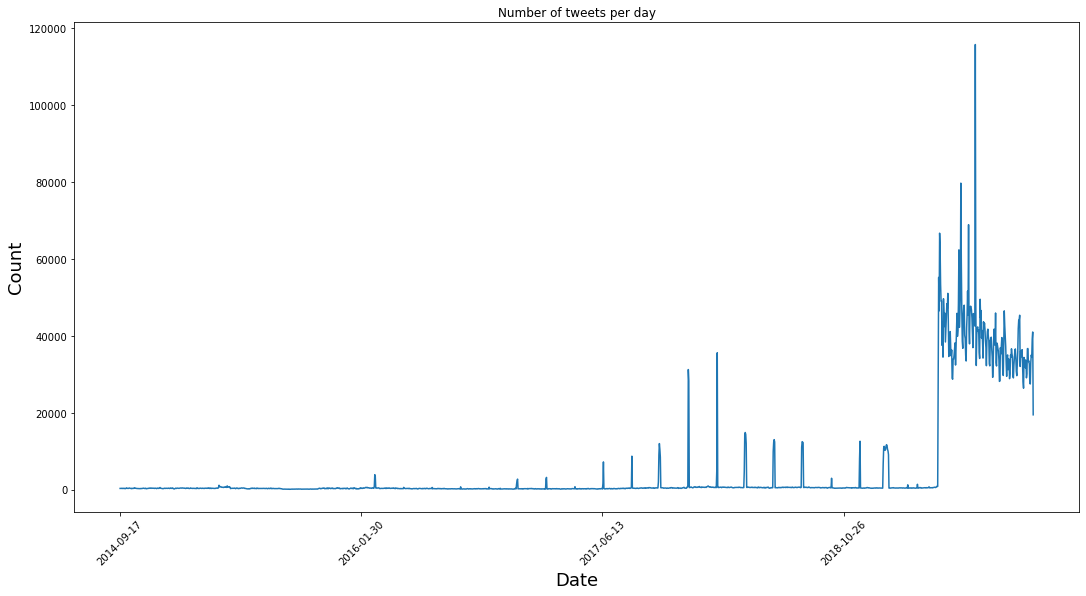
\includegraphics[width=8cm, height=6cm]{Tweet_count}
\label{fig}
\caption{Number of tweet per day}
\end{figure}
We can see an explosion and much more movement since the 23 May 2019. This explosion will start in the middle of our test set. The model might react quite strongly to this major change. Important transformation has to be made to avoid an explosion of the prediction. 

\subsection{BTC-USD Data}\label{AA}
Bitcoin is mainly traded against us dollar. For this specific reason, we choose this currency to know the price of Bitcoin. This dataset comes from Yahoo.\cite{b6} This dataset contains the daily price of Bitcoin in us dollar from 17th September 2014 to 18th May 2022 with 2771 rows and 7 features : \newline
\begin{itemize}
        \item Date : Date
        \item Open : Open price of the day
        \item High : Higher price of the day
        \item Low : Lower price of the day
        \item Close : Closing price of the day
        \item Adj Close : Number of likes
        \item Volume : Total volume of transaction   
\end{itemize}
\medskip
No cleaning was necessary for this dataset.
New variables will be add and calculates based on the variables cited. Further explanations will be given in the methodology section.
\newline
From 2014 to 2022, Bitcoin gained approximately 10'000 percent. From few cent at the beginning to thousand of dollar today, the price of the first cryptocurrency is scrutinize and analysed every days by thousand of people. 

\begin{figure}[H]
	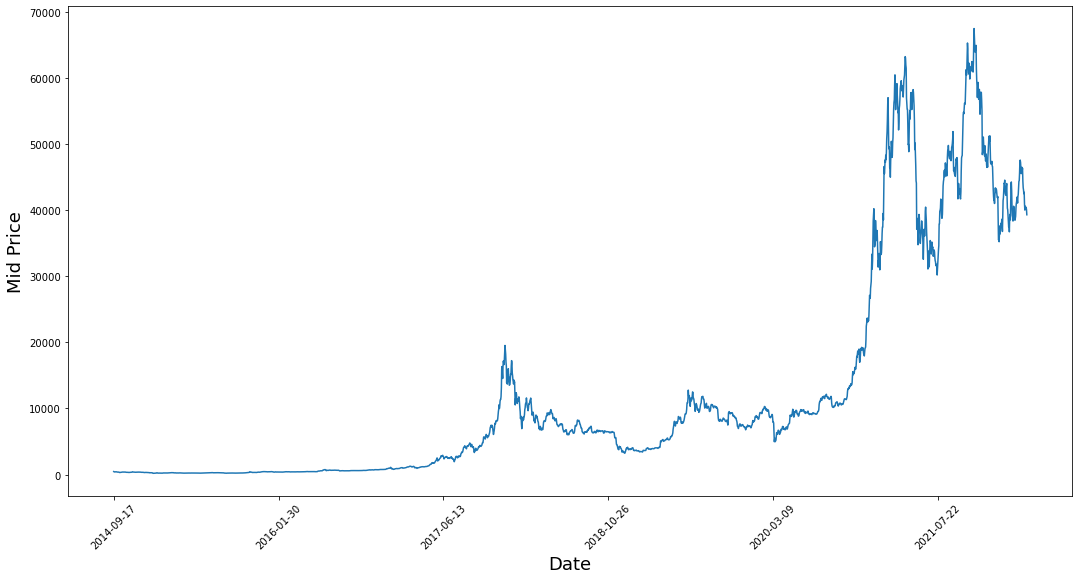
\includegraphics[width=8cm,
 height=6cm]{BTC}
	\label{fig}
	\caption{Price of Bitcooin from 17th September 2014 to 18th May 2022}
\end{figure}

This gigantic growth has been driven by growing interest all around the world. Technical analysis proposed a model to predict Bitcoin over the years. In theory, Bitcoin is supposed to multiply its value by 10 every 3 years. This simple model called the rainbox give indication  if the cryptocurrency is under evaluated or over evaluated. 

\begin{figure}[H]
	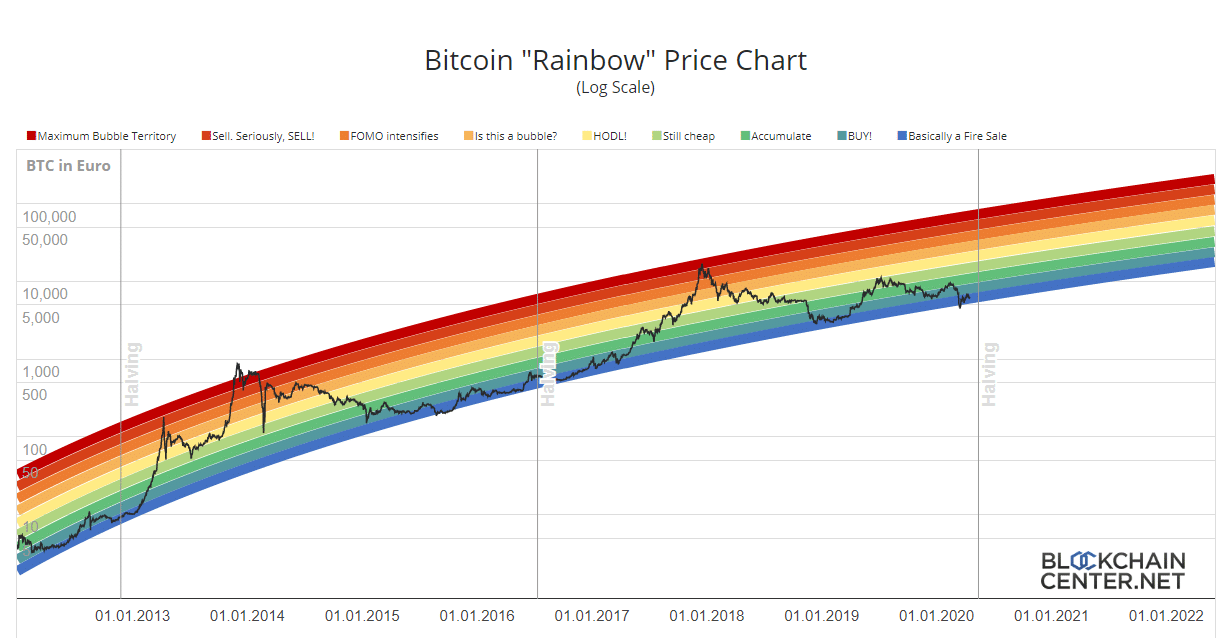
\includegraphics[width=8cm, height=6cm]{BTC_rainbow}
	\label{fig}
	\caption{Bitcoin Rainbow Price Chart}
    \caption*{Source : www.blockchaincenter.net}
\end{figure}

This rainbow chart are telling us something important. Bitcoin will always go up with a rapid growth. This first characteristic is a challenge for our predictive model because it can overfit the data and would not be able to predict a down trend as it is happening since January 2022. 


\section{Methodology}

\subsection{Hypothesis}\label{AA}

The goal is to predict the price of Bitcoin 24 hours later. Predicting the price directly is too hard specially for an asset those value grow in an exponential way and we would not have been able to generalized this model. To avoid this first issue, we implemented a strategy to scale and normalize the data.\newline
\newline
We will predict the price of Bitcoin with the following model. 
First, we will calculate the difference of price of today and tomorrow.
\begin{equation}
difference_{T1} = Price_{T0} - Price_{T1}
\end{equation}
Second, we will turn this difference  into increase or decrease compared to the last current day.
\begin{equation}
y_{T1} = difference_{T1} \div Price_{T0}
\end{equation}
Now, we have the change in price for the next day in percent. This transformation left us with naturally scaled and normalized data.  

\begin{figure}[H]
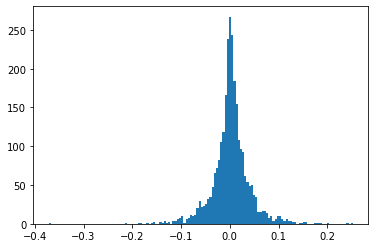
\includegraphics[width=8cm, height=6cm]{I1}
	\label{fig}
	\caption{Daily price difference in percent}
\end{figure}

This new formulation of the problem ensure a better generalization of the algorithm and scaled data. Indeed, the mean is lower than 0.0025.\newline
\newline




\subsection{Import Dataset}\label{AA}
The first step is to import “tweet.csv” data. This data frame contains many tweets from 2009 to 2022 (https://www.kaggle.com/datasets/alaix14/bitcoin-tweets-20160101-to-20190329). After removing non-English character, we run a sentiment analysis on every tweet giving a note between minus 1 to 1. We save this dataset under “tweet-compound.csv”. The second step is to import the data “BTC-USD” that contains volume, opening and closing price in US dollar of bitcoin from  17th September 2014 until 18th of April 2022. 


\subsection{New variables}\label{AA}
In order to improve the accuracy of the model, naturally scale and normalized data, we created new variables in the 2 datasets.\newline
\newline
For the first dataset tweet-compound, we measured the real impact of a tweet with a new variable named “score”. This variable is weighted and includes the compound and the number of like of the tweet. The idea behind is that the more likes a publication obtain, the more impact this tweet will have on the market. Then, we counted the number of tweet per day. The next step is to calculate the daily score difference in percent and the daily count difference in percent. For this 2 new variables we built a 7 days Smoothed Moving Average (SMA), a 14 days SMA and a 21 days SMA. We calculate also the increase or decrease in percent for the next day. \newline
\newline
For the second dataset,we calculate the past daily price difference in percent and the past daily volume difference in percent. Afterwards, we built a 7 days SMA, a 14 days SMA and a 21 days SMA on these 2 new variables.  
To ensure memory and improve the model, we added the previous value over 14 days for these 2 new variables.

\subsection{Splitting and k-fold}\label{AA}
The data are slitted in two different sets: training set and testing set. Considering the few value we had (1850) and how difficult stock market is to predict, we choose 84 percent of data for the training set and 16 percent for the test set. The train set goes from 12 October 2014 to 25 October 2018 and the test set goes from 26 October 2018 to 04 November 2019.\newline
\newline
The DNN model will be feed 10 splits randomly shuffle with a seed to have reproducible result. This ensures us to not overfit the model and build a more generalized model. 


\subsection{Model}\label{AA}
Neural Network (NN) also known as Artificial Neural Network are based and inspired by the neurons in our brain. In 1958, the first NN was created and since, it has been improved many times. Neural Network are often described as black box. There is an input entering a black box (the model) and the black box produce an output. What is happening in the box does not matter and we do not take into consideration the model to explain the output because the mechanism in this black box are too complex. Deep Neural Networks (DNN) are simply neural network with a certain degree of complexity. This model is a powerful tool to build Artificial Intelligence (AI) and big technology companies understood it. Tesla, Uber, Motional and many others are making autonomous vehicles with this algorithm. Currently, level 5 (full automation) has been reach for autonomous vehicle but none have been made available to the general public. \newline
\newline
To predict the daily price difference in percent, we will use a deep RNN network with many layers. 
\begin{figure}[H]
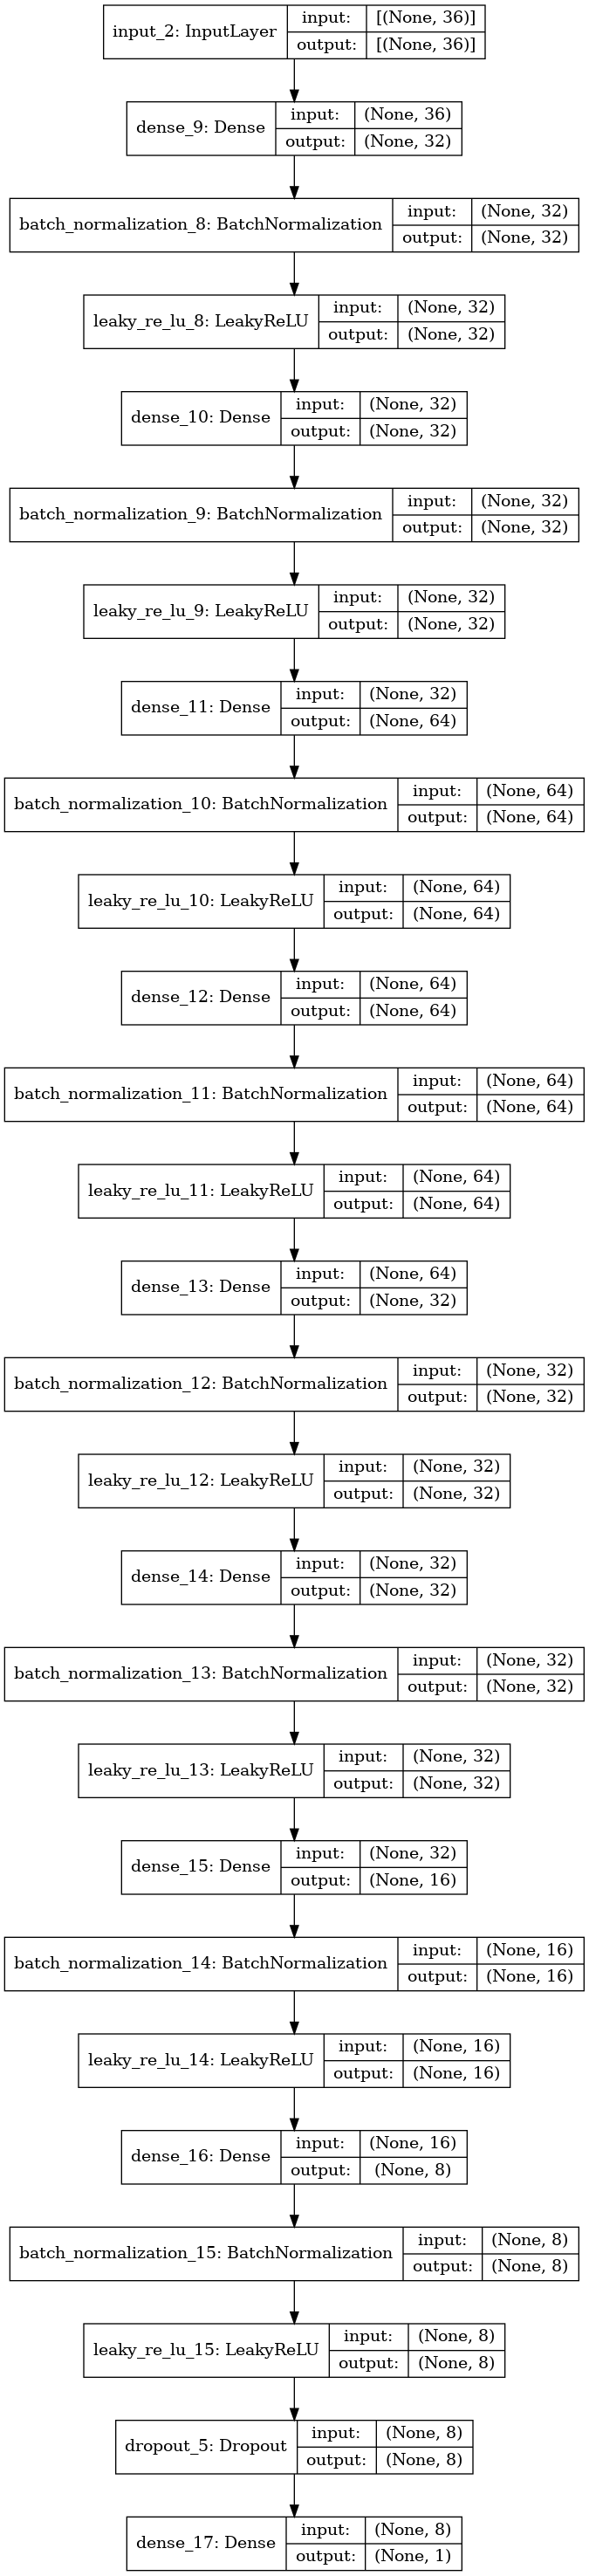
\includegraphics[width=8cm, height=23.5cm]{M1_Model}
	\label{fig}
	\caption{RNN Model}
\end{figure}

The first box, input layer, simply receive all the variables. For the first model, the size is 36 and for the second one 71. This is the only difference between the first and the second model. \newline
\newline
Afterwards, a first dense layer is called and 32 neurons are added. All the input variable are going into each of the 32 neurons. Next, we applied a first batch normalization. This step is crucial for making artificial neural networks quicker and more reliable by normalizing the layers. \newline
\newline
The next step is to add an activation function : LeakyRelU has been chosen. It has the advantage over a simple ReLU function to avoid the vanishing gradient problem and dead neurons. In fact, the LeakyReLU give a small negative value instead of giving 0 for negative input as would do a ReLU.\newline
\newline
We repeat this previous step (Dense, Batch normalization, LeakyReLU) one more time before growing doubling the size of the next dense layer from 32 to 64. We still applied a batch normalization and a LeakyReLU and repeat the process one more time. Now, it is time to scale down our network; we go from 64 to 32 and applied one more time a batch normalization and a LeakyReLU and we repeat the process once. \newline
\newline
Afterwards, the next dense layer is composed of 32 neurons and we had as usual a batch normalization and a LeakyReLU. The process is reapeat over from 32 to 16 and 16 to a dense layer of 8 neurons. In addition, at the end, we add a dropout of 10 percent. This means 1 neurons of of the 8 will be dropped during the training phase. The techniques help us to build more generalized tweet and not over fit the data. On average, it makes our RNN resilient. \newline
\newline
It is important to choose n power 2 neurons to optimize the process. After building this model, we have to decide few hyperparameter \begin{itemize}
        \item initial learning rate 
        \item decay step
        \item decay rate
\end{itemize}
\medskip
Through a lot of testing, we choose 0.0015 for the learning rate, 1500 for the decay step and 0,95 for the decay rate.\newline
\newline
Our first model will only use the historical price and volume of Bitcoin while we will add the data on tweets with the senetiment analysis for the second model. There is no need to scale the data for the first model because all variable have aproximately the same scale. However, for the second model, we scaled our data to have a better prediction. 



\section{Implementation}
\subsection{Programm version}\label{AA}
This project was programmed with the Jupyter Notebook
(.ipynb), the program runs in python version 3.10.4. This
program uses many python libraries such as :\newline
\begin{itemize}
        \item Pandas : version 1.2.4
        \item Numpy : version 1.2.4
        \item TensorFlow  : version 2.8.0
        \item VaderSentiment : version 3.3.2
\end{itemize}
\medskip
Our project has been developed in 2 parts for time reasons. The first program will give a compound to each tweet with a sentiment analyser; this first step take a lot of ressources. The second program will clean the dataset and build the different models.

\subsection{Files}\label{AA}
There is 2 ipynb file and 3 data files. The notebook "twitter-analyse.ipynb" will load the data file "tweets.csv" and perform a sentiment analysis and store the new dataset as "tweet-compound.csv". The notebook "Final-model.ipynb" will load the data set "BTC-USD" and the data set "tweet-compound.csv".


\section{Results}
\subsection{Naive models}\label{AA}
The goal of this study is to predict for the next day the difference of price for Bitcoin with the help of sentiment analysis of tweets. Based on the model described above and tuned with the hyperparameters discussed earlier, the model display interesting result.  
\newline
\newline
In order to have a first good point of comparison, we will construct 2 naive models. They have the advantage of being inexpensive to develop and run. The disadvantage is that it overlooks any possible causal relationships beneath the projected variable.
The purpose of the first one will be to forecast the price of Bitcoin within a day while the purpose of the second one will be to have the lowest RMSE.
\newline

The first naive model is described as follow : 

\begin{equation}
y_{T1} = y_{T0}
\end{equation}
The increase of y percent for the next day is the increase of y percent of today. The first milestone of this project is to beat this simplistic model. 
 
\begin{figure}[H]
\includegraphics[width=8cm, height=6cm]{NM_FInal}
	\label{fig}
	\caption{First naive model}
\end{figure}

Indeed, with an RMSE of 0.056, this naive model. 
\newline

The second naive model but not useful to predict the price of Bitcoin follow this rule :
\begin{equation}
y_{T1} = 0
\end{equation}
The increase of y percent for the next day always equal to 0. Even more simpler than the previous naive model, it show a quite strong RMSE of only 0.41.
\newline

\subsection{First model}\label{AA}
The main goal of this first model is to beat the first naive model. If this model show a lower RMSE, this model has produce a better prediction than the first naive model. In order to choose the right number of epoch and not overfit the data we will compare the train loss rate and the validation loss rate.

\begin{figure}[H]
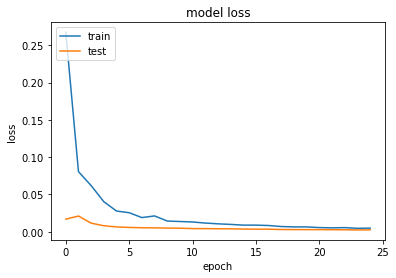
\includegraphics[width=8cm, height=6cm]{M1_loss}
	\label{fig}
	\caption{Frist model train/test loss}
\end{figure}


Surprisingly, since epoch one, the test loss rate is lower than the train loss rate. This unexpected result deserve further explanations. \newline
\newline
The first explanation concern regularization applied to the train set such as dropout. Indeed, the dropouts in our model are applied to the training but not during the validation. Regularisation methods are useful to improve the validation loss while decrease the loss of training. This particular situation can lead to lower loss for testing than for training. 
In our case, a dropout of only 10 percent is very low. It doest not seem to explain thus huge differenced observed. \newline
The second explantion concerned when the training loss and validation loss is compute. \newline
\newline Based on the graphic above, we need to choose the number of epoch in order to not overfit the data to have a generalized model. An epoch of 12 is optimal to fill this purpose. This also produce a visually nice prediction that follow movement.\newline
\newline The prediction made with this first model without including twitter's data is actually capable to beat the first naive model with an RMSE of 0.0425.

\begin{figure}[H]
\includegraphics[width=8cm, height=6cm]{M1_FInal}
	\label{fig}
	\caption{Second model prediction}
\end{figure}

We can see the prediction follow quite randomly the real value but in a shorter range; from minus 2 percent to 5 percent. The increase in percent for the next day on average based on this model is slightly above 0 for this period of time. 

\begin{figure}[H]
\includegraphics[width=8cm, height=6cm]{M1_FInal_chart}
\label{fig}
\caption{Second model final prediction}
\end{figure}

This last figure for the first model show the real prediction in price for Bitcoin over the period. 


\subsection{Second model}\label{AA}
For this second model, we add our data with twitter and sacled the test and train data. Again, we need to choose the number of epoch for our model. We need to not overfit  and to generalize. 

\begin{figure}[H]
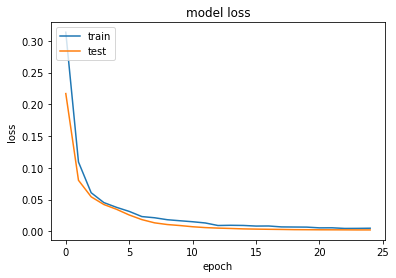
\includegraphics[width=8cm, height=6cm]{M2_loss}
\label{fig}
\caption{Second model train/test loss}
\end{figure}

This loss value of the test and train is much more normal than the previous one. However, the test loss value is still lower since the first epoch. The second explanations for this difference is the training loss value is calculate through the entire epoch while the test vall loss is calculat at the end. Concretely, the train loss value is calculate half an epoch earlier than the test value loss. If we look again at our graphic above and move the blue line to the left by 0.5, the result are better and it explain the difference.\newline
\newline
After few test and based on the model above, an epoch of 8 would not overfit the data and has a good test loss value.\newline

\begin{figure}[H]
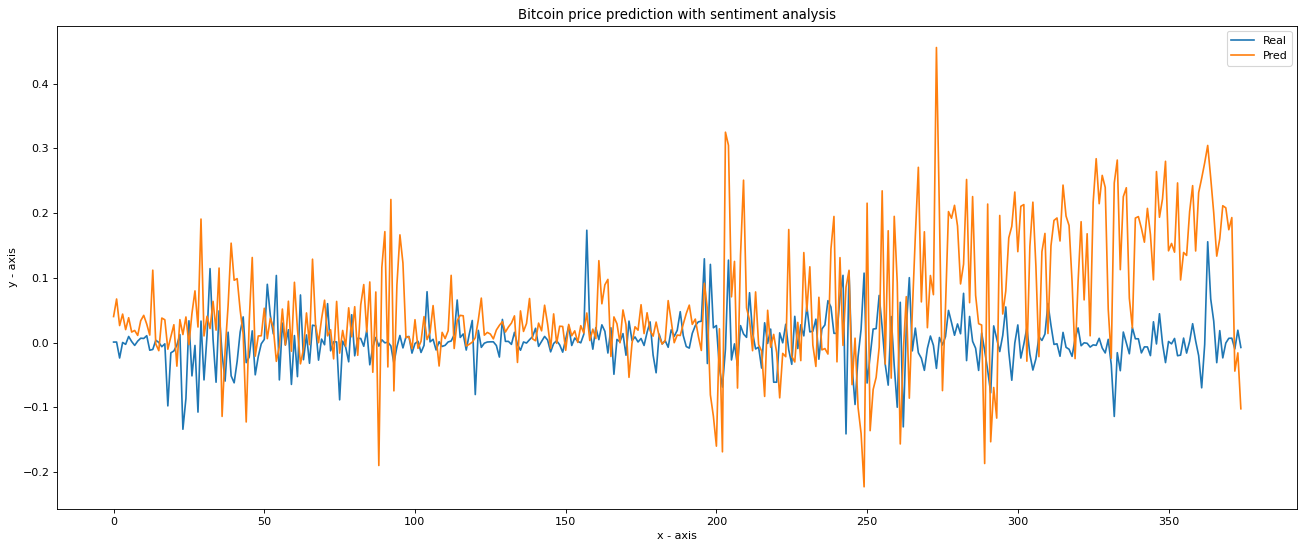
\includegraphics[width=8cm, height=6cm]{M2_Final}
\label{fig}
\caption{Second model prediction}
\end{figure}

After many trial and parameter tuning, this this the best model we got. Even by removing the daily change in percentage in the number of tweets or the daily change in percentage in volume, the prediction was stil worse than the other one. With an RMSE of 0,12, this model is definitely  not able to beat the naive model.\newline
\newline
The first thing to not is this prediction is more volatile than the other one. The range of the prediction is from minus 0,2 to 0,45. In addition, from the number 200 (that correspond to 14th May 2019), the model explode and there is an obvious trend upside. \newline
\newline
From the 14th of May, many variables such as the daily change in percentage in volume and the daily change in percentage in the number of tweets show more volatility. This situation leads to more volatility in the prediction as well. Before the 14th of May, the model never encountered such extreme value and volatile value. 

\begin{figure}[H]
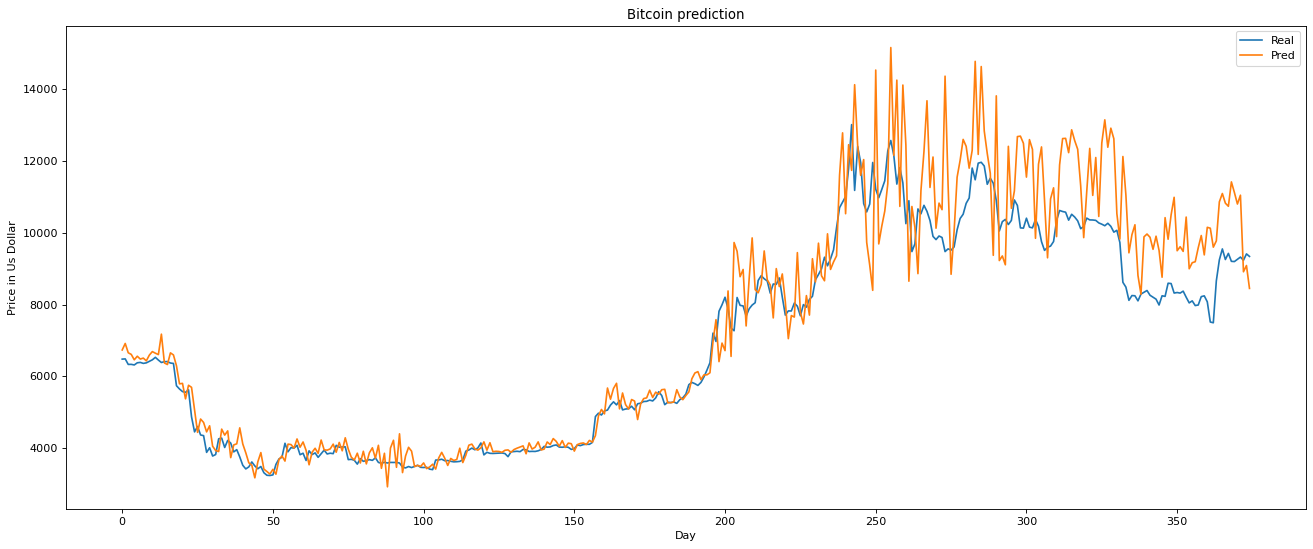
\includegraphics[width=8cm, height=6cm]{M2_Final_chart}
\label{fig}
\caption{Second model final prediction}
\end{figure}

This last figure for the second model show the real prediction in price for Bitcoin over the period.\newline
\newline
We would like to emphasize the fact we train our model on the daily price different in percent. Henceforth, it is evident to compare the prediction to the real daily price change in percent. The chart showing the real price of BItcoin with the prediction of the price of Bitcoin is purely for visual purpose. The Fig 9 and the Fig 12 should not be used to evaluate the models.


\section{Conclusion}
Stock prediction have been up for decades, but sentiment analysis coupled with other metrics of social media had gain in interest on the last 2 years after the boom of cryptocurrency  and the GameStop stock. A model with even a 51 percent prediction would make thousand of dollar of profit. This only works if one actor posses it an the others do not know yet and are not able to counter it with another AI.\newline
\newline
Using a RNN have proved it is possible to beat the first naive model with only historical price of Bitcoin. However, the second model with twitter's data showed poor result. We are convinced an different approach of the problem but more importantly  a different time where the model is train would result in significant improvement of our second model.\newline
\newline
Further exploration could be made also on the type of neural network.In finance, past performance are not indicator of a future performance. In other words, historical data should not be able to predict anything in the future. However, the exact same hypothesis exist on the opposite. Indeed, Long-Short-Term-Memory (LSTM) networks are based this strong opposite hypothesis. LSTM network might produce a better prediction specially for stock market data. It has the specificity to remember informations over the long run. This advantages would result in a better prediction.



\begin{thebibliography}{00}
\bibitem{b1} D. R. Pant, P. Neupane, A. Poudel, A. K. Pokhrel and B. K. Lama, "Recurrent Neural Network Based Bitcoin Price Prediction by Twitter Sentiment Analysis," 2018 IEEE 3rd International Conference on Computing, Communication and Security (ICCCS), 2018, pp. 128-132, doi: 10.1109/CCCS.2018.8586824
\bibitem{b2} Stenqvist, E., and Lonno, J. 2017. Predicting Bitcoin price fluctuation with Twitter sentiment analysis.
\bibitem{b3}Kolasani, S. and Assaf, R. 2020 Predicting Stock Movement Using Sentiment Analysis of Twitter Feed with Neural Networks. Journal of Data Analysis and Information Processing
\bibitem{b4} Weiling Chen, Chai Kiat Yeo, Chiew Tong Lau, Bu Sung Lee, Leveraging social media news to predict stock index movement using RNN-boost
\bibitem{b5}Kaggle, https://www.kaggle.com/datasets/alaix14/bitcoin-tweets-20160101-to-20190329, Twitter Data
\bibitem{b6} Vader, https://github.com/cjhutto/vaderSentiment, vaderSentiment
\bibitem{b7}Yahoo, https://finance.yahoo.com/quote/BTC-USD/, Bitcoin USD BTC-USD
\bibitem{b8} https://www.tensorflow.org/?hl=fr

\end{thebibliography}
\end{document}
